\documentclass[a4paper,5pt]{amsbook}
%%%%%%%%%%%%%%%%%%%%%%%%%%%%%%%%%%%%%%%%%%%%%%%%%%%%%%%%%%%%%%%%%%%%%

%\usepackage{booktabs}
\usepackage{graphicx}
%\usepackage{multicol}
%\usepackage{textcomp}
%\usepackage{systeme}
%\usepackage{amssymb}
%\usepackage[]{amsmath}
%\usepackage{subcaption}
%\usepackage[inline]{enumitem}
%\usepackage{gensymb}

%%%%%%%%%%%%%%%%%%%%%%%%%%%%%%%%%%%%%%%%%%%%%%%%%%%%%%%%%%%%%%

\newcommand{\sen}{\,\mbox{sen}\,}
\newcommand{\tg}{\,\mbox{tg}\,}
\newcommand{\cosec}{\,\mbox{cosec}\,}
\newcommand{\cotg}{\,\mbox{cotg}\,}
\newcommand{\tr}{\,\mbox{tr}\,}
\newcommand{\ds}{\displaystyle}
\newcommand{\ra}{\rightarrow}

%%%%%%%%%%%%%%%%%%%%%%%%%%%%%%%%%%%%%%%%%%%%%%%%%%%%%%%%%%%%%%%%%%%%%%%%

\setlength{\textwidth}{16cm} \setlength{\topmargin}{-1.7cm}
\setlength{\textheight}{25cm}
\setlength{\leftmargin}{1.2cm} \setlength{\rightmargin}{1.2cm}
\setlength{\oddsidemargin}{0cm}\setlength{\evensidemargin}{0cm}

%%%%%%%%%%%%%%%%%%%%%%%%%%%%%%%%%%%%%%%%%%%%%%%%%%%%%%%%%%%%%%%%%%%%%%%%

% \renewcommand{\baselinestretch}{1.6}
% \renewcommand{\thefootnote}{\fnsymbol{footnote}}
% \renewcommand{\theequation}{\thesection.\arabic{equation}}
% \setlength{\voffset}{-50pt}
% \numberwithin{equation}{chapter}

%%%%%%%%%%%%%%%%%%%%%%%%%%%%%%%%%%%%%%%%%%%%%%%%%%%%%%%%%%%%%%%%%%%%%%%

\begin{document}
\thispagestyle{empty}
\pagestyle{empty}
\begin{minipage}[h]{0.14\textwidth}
	
\includegraphics[scale=0.24]{../ufgd.png}
\end{minipage}
\begin{minipage}[h]{\textwidth}
\begin{tabular}{c}
{{\bf UNIVERSIDADE FEDERAL DA GRANDE DOURADOS}}\\
{{\bf C\'alculo Diferencial e Integral --- Lista 13}}\\
{{\bf Prof.\ Adriano Barbosa}}\\
\end{tabular}
\vspace{-0.45cm}
%
\end{minipage}

%------------------------

\vspace{1cm}
%%%%%%%%%%%%%%%%%%%%%%%%%%%%%%%%   formulario  inicio  %%%%%%%%%%%%%%%%%%%%%%%%%%%%%%%%
\begin{enumerate}
    \vspace{0.5cm}
    \item Encontre a antiderivada mais geral para as fun\c{c}\~oes abaixo:
        \begin{enumerate}
            \item $f(x)=x-3$
            \item $f(x)=\ds\frac{1}{2}+\frac{3}{4}x^2-\frac{4}{5}x^3$
            \item $f(x)=(x+1)(2x-1)$
            \item $f(x)=\ds\frac{1+x+x^2}{\sqrt{x}}$
            \item $f(x)=2\sen{x}-\sec^2{x}$
        \end{enumerate}

    \vspace{0.5cm}
    \item Encontre $f$ tal que:
        \begin{enumerate}
            \item $f''(x)=20x^3-12x^2+6x$
            \item $f'(x)=1+3\sqrt{x}$, $f(4)=25$
            \item $f'(x)=\sqrt{x}(6+5x)$, $f(1)=10$
            \item $f''(x)=2+\cos{x}$, $f(0)=-1$, $f(\pi/2)=0$
        \end{enumerate}

    \vspace{0.5cm}
    \item O gr\'afico de uma fun\c{c}\~ao $f$ \'e dado em cada item. Determine qual dos
        gr\'aficos $a$, $b$ ou $c$ \'e a antiderivada de $f$.
        \begin{figure}[h]
            \centering
            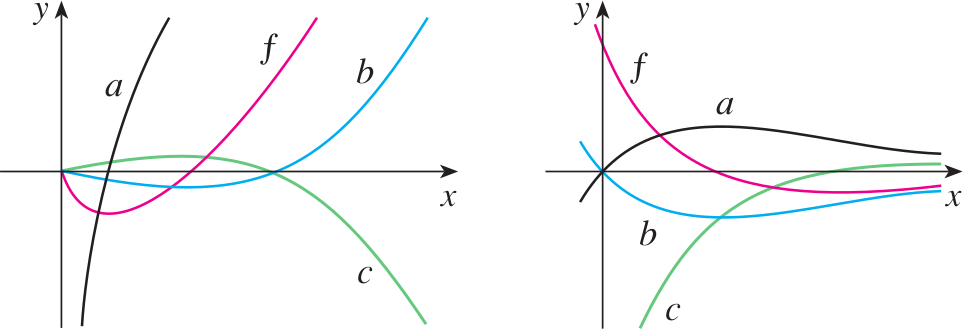
\includegraphics[width=0.6\textwidth]{lista-13-fig1.png}
        \end{figure}

    \vspace{0.5cm}
    \item Como deve ser o gr\'afico de uma antiderivada de $f$ se o gr\'afico de
        $f$ for
        \begin{figure}[h]
            \centering
            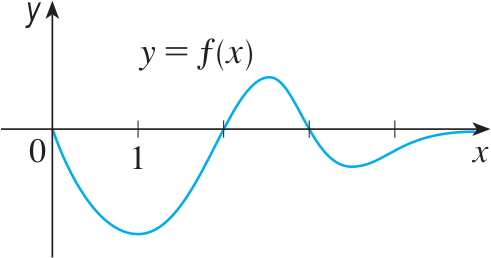
\includegraphics[width=0.3\textwidth]{lista-13-fig2.png}
        \end{figure}

    \vspace{0.5cm}
    \item Estime a \'area abaixo do gr\'afico de $f(x)=\cos{x}$ de $x=0$ at\'e
        $x=\ds\frac{\pi}{2}$ usando quatro ret\^angulos aproximantes usando os
        extremos direitos dos subintervalos. Repita o c\'alculo usando os
        extremos esquerdos dos subintervalos.

    \vspace{0.5cm}
    \item A velocidade de um corredor aumenta regularmente durante os tr\^es
        primeiros segundos de uma corrida. Sua velocidade em intervalos de
        meio segundo \'e dada pela tabela abaixo. Encontre as estimativas
        superior e inferior para a dist\^ancia que ele percorreu durante esses
        tr\^es segundos.

        \vspace{0.3cm}
        \begin{center}
        \begin{tabular}{|c|c|c|c|c|c|c|c|}
            \hline
            $t$ (s) & 0 & 0,5 & 1,0 & 1,5 & 2,0 & 2,5 & 3,0 \\
            \hline
            $v$ (m/s) & 0 & 1,9 & 3,3 & 4,5 & 5,5 & 5,9 & 6,2 \\
            \hline
        \end{tabular}
        \end{center}


\end{enumerate}

\end{document}
